
\documentclass{article}

\usepackage{graphicx}
\usepackage[centerlast,small,sc]{caption}
\usepackage{alltt}
\usepackage{url}
\usepackage{tabularx}
%\usepackage{ngerman}
\usepackage{longtable}
\usepackage[utf8]{inputenc}
\usepackage[italian]{babel}

\newenvironment{prettytablex}[1]{\vspace{0.3cm}\noindent\tabularx{\linewidth}{@{\hspace{\parindent}}#1@{}}}{\endtabularx\vspace{0.3cm}}
\newenvironment{prettytable}{\prettytablex{l X}}{\endprettytablex}



\title{\huge\sffamily\bfseries Descrizione del sistema e Analisi del Rischio}
\author{Nicolò Marchi \and Alessandro Gottoli \and Mattia Peretti}
\date{\today}


\begin{document}
\maketitle

\tableofcontents
\listoffigures
\pagebreak


\section{Descrizione del Sistema}

\subsection{Panoramica del sistema}

L'assegnamento per il laboratorio di Sicurezza delle Reti consisteva nell'implementazione di una Certification Authority (in seguito, CA) riguardante una fittizia compagnia di nome \emph{iMovies}, che vuole offrire ai suoi clienti dei servizi basati su PKI (Public Key Infrastructure).
Le direttive per l'implementazione di tale CA sono descritte dal libro di testo\footnote{``Applied Information Security'' di David Basin, Patrick Schaller e Micheal Schl\"apfer.} adottato.

---Possibile descrizione PKI

La nostra implementazione di iMovies permette agli utenti (già inseriti nel database fornito) la creazione e la firma di certificati che verranno poi usati per la comunicazione sicura tramite e-mail.

L'architettura del sistema è composta da due parti:
\begin{itemize}
\item \textbf{serverIMovies} - una macchina virtuale a 64 bit con sistema operativo \emph{Ubuntu Server 12.04 server} provvista del contenitore servlet open source \emph{Apache Tomcat 7.0.26}.
\item \textbf{clientIMovies} - una macchina virtuale a 64 bit con sistema operativo \emph{Ubuntu Server 12.04 client} con doppia utenza (administrator e client).
\end{itemize}

La web application è stata scritta utilizzando il framework Java Server Faces (JSF) per permettere una maggiore attenzione al backend Java attraverso una più facile implementazione del frontend grafico composto da pagine xhtml (create utilizzando le librerie di componenti grafici \emph{Primefaces}\footnote{Per maggiori informazioni, http://www.primefaces.org}.).

Per la gestione del database ci si è affidati al  Relational Database Management System MySql.

Per quanto riguarda la creazione, la firma, la revoca, e tutte le operazioni di gestione dei certificati ci si è affidati al toolkit \emph{OpenSSL}\footnote{Implementazione open-source dei protocolli SSL/TLS.}. 

Infine, per gli archivi di backup dei dati è stato usato il semplice tool \emph{tar}, presente in ogni distribuzione Unix. Per lo scheduling dei backup è stato usato il tool \emph{cron}, e per il download dei backup ci siamo affidati a   

%This description should provide a high-level
%overview of the system, e.g., suitable for managers, that complements
%the more technical description that follows.


\subsection{Funzionalità del Sistema}
\subsubsection*{Login}
\begin{figure}[h!]
\centering
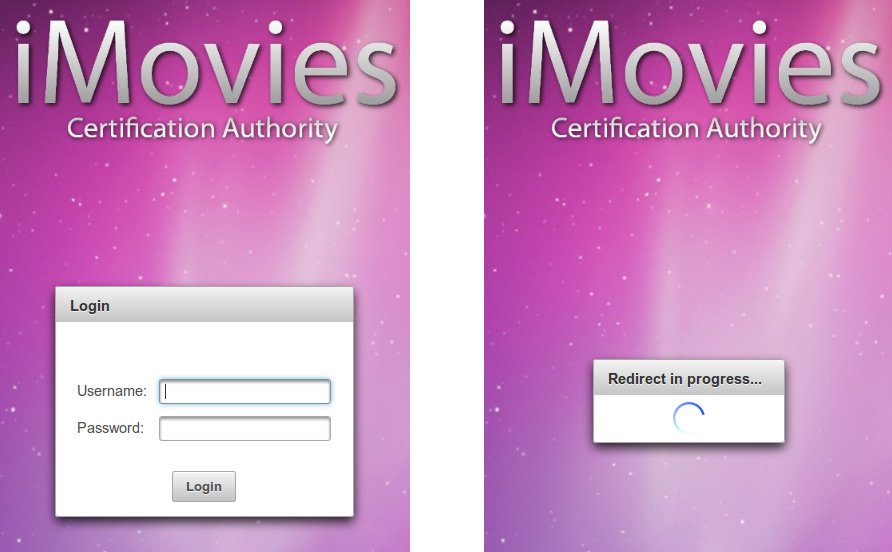
\includegraphics[width=\textwidth]{img/login}
\caption{Differenza tra il login che viene mostrato al cliente (immagine a sinistra) e il login automatico tramite certificato per l'amministratore.}
\end{figure}
Il sistema offre principalmente due possibilità di login. Una possibilità consiste nel connettersi al portale attraverso un certificato PKCS\#12 riconosciuto dalla CA iMovies, che permette di bypassare il controllo delle credenziali nel database (dato che si presume che il certificato sia in mano al proprietario dello stesso).
\par La seconda modalità consiste in un canonico form di login nel quale l'utente è chiamato ad inserire lo username e la password. Per quest'ultimo campo, verrà calcolato il corrispondente hash SHA-1 e tale valore sarà utilizzato nel confronto con gli hash delle password salvati nel database.
\subsubsection*{Modifica informazioni personali}
\begin{figure}[h!]
\centering
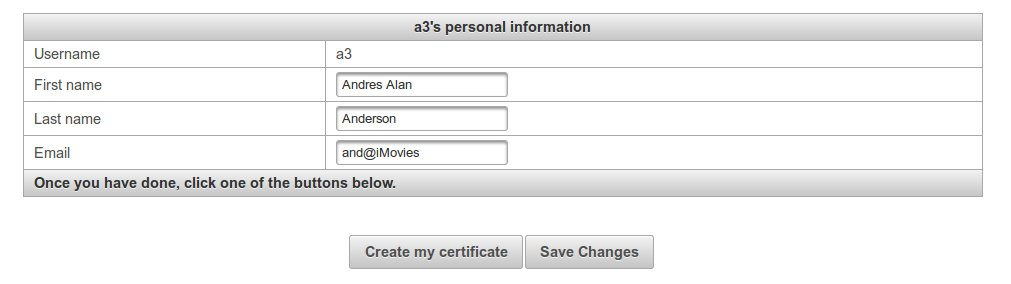
\includegraphics[width=\textwidth]{img/edit}
\caption{Le tabella contenente le informazioni personali modificabili dell'utente \emph{a3}.}
\end{figure}
Il portale offre agli utenti la possibilità di modificare le informazioni personali precedentemente salvate nel database. Si possono modificare tutti i campi, ad eccezione del campo username, che è fisso e ha il ruolo di primary key nella tabella relativa agli utenti nel database.
\subsubsection*{Rilascio di certificati}
Ad ogni utente viene fornita la possibilità di creare certificati. Alla creazione di un certificato viene generata una chiave privata con crittografia a 4096 bit e crittata con DES3 e una password inserita dall'utente. Dopodiché viene generato e firmato il certificato relativo, con i dati dell'utente salvati nel database.
\subsubsection*{Revoca dei certificati}
Nella sezione di management dei certificati viene fornita la possibilità di revocare selettivamente i certificati dell'utente. Quando un certificato viene revocato, viene generata nuovamente la Certificate Revocation List della Certificate Authority.
\subsubsection*{Download dei certificati}
Viene fornita la possibilità di scaricare i certificati e le relative chiavi private in formato PKCS\#12. Quando si richiede il download del certificato il sistema richiederà all'utente la password usata durante la creazione della chiave privata, e una nuova password che sarà usata per l'esportazione del certificato PKCS\#12. QUest'ultima password dovrà essere inserita quando si importerà il certificato all'interno di un browser.
\subsubsection*{Eliminazione dei certificati}
\begin{figure}[h!]
\centering
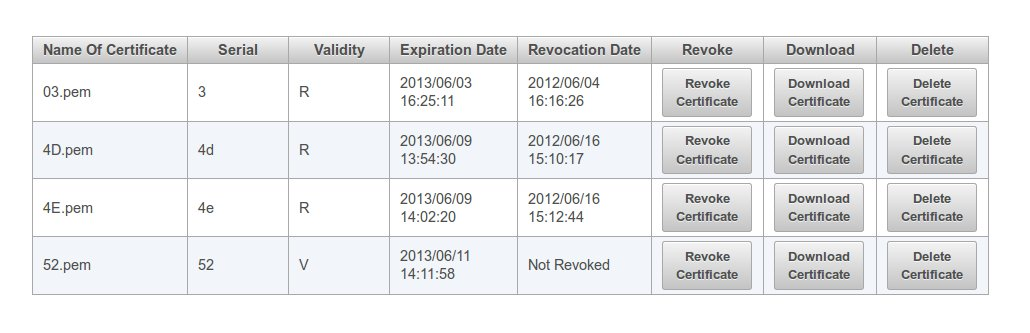
\includegraphics[width=\textwidth]{img/revokedownload}
\caption{Tabella per il download, la revoca e l'eliminazione dei certificati.}
\end{figure}
Quando un utente sceglie di rimuovere un certificato, innanzi tutto quest'ultimo verrà revocato; dopodiché verrà eliminata la chiave privata associata al certificato, e il certificato stesso.
\subsubsection*{Amministrazione del portale}
\begin{figure}[h!]
\centering
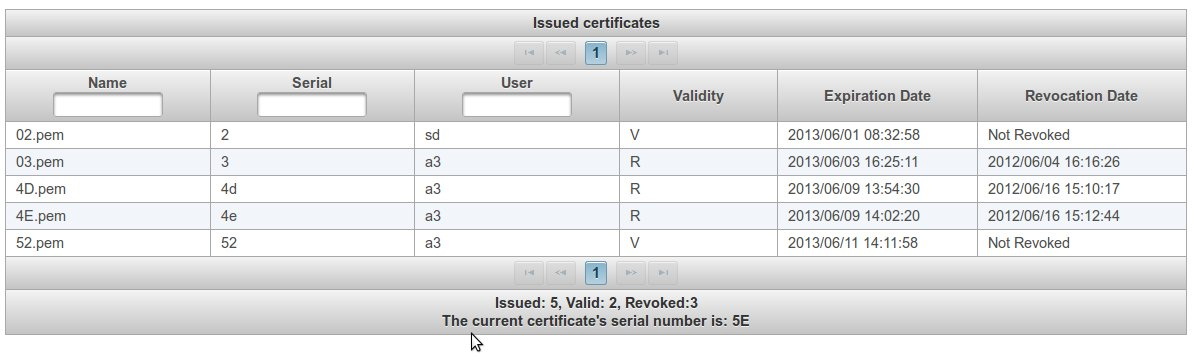
\includegraphics[width=\textwidth]{img/certs}
\caption{Tabella per la visualizzazione di tutti i certificati rilasciati con contatori e prossimo serial number.}
\end{figure}
L'amministratore del portale accede al frontend di amministrazione solamente con un certificato PKCS\#12 già in suo possesso. Attraverso le pagine dell'area amministrativa,  l'amministratore può vedere quanti e quali certificati sono stati rilasciati, quanti e quali certificati sono stati revocati, e il valore corrente del serial number\footnote{il valore del numero esadecimale che verrà assegnato al prossimo certificato generato}.
\par Inoltre viene effettuato un log di tutti gli accessi al sito, compresi gli accessi effettuati passando attraverso le backdoor.
\subsubsection*{Backup dei dati}
Il sistema esegue un periodico backup di tutte le chiavi private e di tutti i certificati. I backup sono in realtà due, uno totale che viene eseguito ogni settimana il venerdì alle ore 11.00, mentre un backup incrementale che viene eseguito tutte le ore al minuto 40. In entrambi i casi viene generato un archivio con il comando Unix ``tar''.
\par Vi è poi un server ftp che permette ad un amministratore di scaricare da remoto i backups. L'accesso da ftp è limitato solamente alla cartella ove vi sono i backups.
\subsection{Componenti e Sottosistemi}
\subsubsection*{Java Server Faces}
Come già accennato, per l'implementazione del portale è stata usata la tecnologia di Java Server Faces. JSF, acronimo di Java Server Faces può essere considerata un framework per lo sviluppo di web application basate su Java. \'E basato sul design pattern architetturale Model-View-Controller (MVC) ed è descritto da un documento di specifiche (JSR 127) alla cui stesura hanno partecipato aziende quali IBM, Oracle Corporation, Siemens e Sun Microsystems. Il suo scopo è di semplificare lo sviluppo dell'interfaccia utente (UI) di una applicazione Web.
\par A grandi linee il funzionamento del framework JSF si basa su un file di configurazione XML ({\tt faces-config.xml}) in cui vengono definite le viste (sostanzialmente pagine JSP che sfruttano la \emph{taglibrary faces}) e i controllori. Le singole implementazioni sfruttano una servlet di base {\tt FacesServlet} o un filtro il cui mapping è normalmente {\tt /faces/*} o {\tt *.faces}. La {\tt FacesServlet} deve essere registrata nel file XML ({\tt web.xml}) della web application.
\subsubsection*{PrimeFaces}
\begin{figure}[h!]
\centering

\includegraphics[width=.5\textwidth]{img/prime}
\caption{Il logo delle librerie Primefaces.}
\end{figure}
Le librerie Primefaces costituiscono una serie di componenti grafici utilizzabili all'interno di una web application Jsf.
PrimeFaces è una suite open source utilizzabile con il framework Java Server Faces, esplicitamente pensata per realizzare i componenti presentazionali di una applicazione web enterprise: editor HTML, finestre di dialogo, meccanismi per l'auto-completamento, grafici e calendari, drag \& drop, integrazione di mappe google e molto altro.
\par La suite offre supporto sia ad ajax che al rendering parziale delle pagine web, grazie ad una integrazione nativa con {\tt jquery}. L'aspetto grafico dei componenti si basa su {\tt JQuery UI}: è quindi possibile personalizzarlo attraverso lo skin framework \emph{Theme Roller}, o utilizzare un discreto insieme di temi predefiniti. Da segnalare infine la presenza di uno \emph{User Interface Kit} per la realizzazione di applicazioni Web orientate ai dispositivi mobili (iPhone, Android, etc.), di semplice e veloce configurazione.
%Per tale motivo, in unione con gli ottimi componenti grafici forniti dalle librerie Primefaces, la nostra scelta è ricaduta su questo tipo di tecnologia.

\subsubsection*{Macchine Virtuali}
Le macchine virtuali create sono due, create con il software open source \emph{VirtualBox}, e sono suddivise in macchina server e macchina client.
\par La macchina client consiste in un'installazione della distribuzione Linux \emph{Ubuntu 12.04 LTS} per architetture \emph{amd64}. Nella macchina sono presenti due utenti principali:
\begin{enumerate}
\item utente \emph{admin}: è l'utente che funge da admin del portale iMovies. Nell'utenza vi è già installato il certificato PKCS\#12 relativo all'amministratore che permette il login rapido alla sezione di amministrazione del portale, un client ftp (più precisamente FileZilla) per il download dei backups da remoto.
\item utente \emph{client}: l'utente client consiste invece in un semplice utente, senza grosse particolarità.
\end{enumerate} 
\par La macchina server invece consiste in un'installazione della distribuzione Linux \emph{Ubuntu Server 12.04 LTS} sempre per architetture \emph{amd64}.
Al suo interno troviamo installati tutti i servizi utili al mantenimento e all'esecuzione del portale.
\par Le macchine virtuali si trovano connesse tra loro in una rete interna, con assegnati come indirizzi IP 192.168.1.11 per la macchina server, mentre 192.168.1.10 per la macchina client.
\subsubsection*{Web Server}
Per poter utilizzare le Java Server Faces, abbiamo dovuto scegliere (in maniera quasi obbligata) il web server \emph{Apache Tomcat 7.0}, ultima versione del noto web container.
Tomcat è un contenitore servlet open source sviluppato dalla Apache Software Foundation. Implementa le specifiche Java Server Pages (JSP) e Servlet, fornendo quindi una piattaforma per l'esecuzione di applicazioni Web sviluppate nel linguaggio Java. La sua distribuzione standard include anche le funzionalità di web server tradizionale, che corrispondono al prodotto Apache.
\subsubsection*{test}

 --------------------not finished
List all system components, subdivided, for example, into
  categories such as platforms, applications, data records, etc. For
  each component, state its relevant properties.


\subsection{Interfacce}
\subsubsection*{login.xhtml}
La pagina di login si presenta molto semplice, con un semplice form di login dove inserire username e password. Dalla pagina di login si passa sempre e comunque, anche se si ha un certificato PKCS\#12 riconosciuto. In quest'ultimo caso nella pagina viene effettuato il controllo del certificato e il redirect alla pagina di amministrazione (in caso di certificato dell'admin) o nella pagina dell'user, con i dati dell'utente.
\subsubsection*{user.xhtml}
La pagina consiste in una semplice pagina di benvenuto dove vi è presente un menù di navigazione e un semplice messaggio di benvenuto. Da questa pagina l'utente può muoversi tra tutte le funzionalità del portale.
\subsubsection*{edit.xhtml}
\'E la pagina 
\subsubsection*{admin.xhtml}
Specify  all interfaces and  information flows, from the technical as well as from the
  organizational point of view.

\subsection{Backdoors}

Describe the implemented backdoors. {\bfseries Do not add
    this section to the version of your report that is handed over to
    the team that reviews your system!}

\subsection{Materiale Aggiuntivo}

You may have additional sections according to your needs.


\section{Risk Analysis and Security Measures}

\subsection{Information Assets}

Describe the relevant assets and their required security
  properties. For example, data objects, access restrictions,
  configurations, etc.

\subsection{Threat Sources}

Name and describe potential threat sources.

\subsection{Risks and Countermeasures}

List all potential threats and the
  corresponding countermeasures. Estimate the risk based on 
  the information about the threat, the threat sources and the 
  corresponding countermeasure. For this purpose, use the following three
  tables.

%\subsubsection{Tools}

\begin{center}
\begin{tabular}{|l|l|}
\hline
\multicolumn{2}{|c|}{\bf Impact} \\
\hline
Impact & Description \\
\hline
\hline
High   & \hspace*{20pt}\ldots \\
\hline
Medium & \hspace*{20pt}\ldots \\
\hline
Low   & \hspace*{20pt}\ldots \\
\hline
\end{tabular}
%
%\vspace{5mm}
%
%\noindent \hspace*{10pt}
\begin{tabular}{|l|l|}
\hline
\multicolumn{2}{|c|}{\bf Likelihood} \\
\hline
Likelihood & Description \\
\hline
\hline
High   & \hspace*{20pt}\ldots \\
\hline
Medium & \hspace*{20pt}\ldots \\
\hline
Low   & \hspace*{20pt}\ldots \\
\hline
\end{tabular}
\end{center}

\vspace{5mm}

\begin{center}
\begin{tabular}{|l|c|c|c|}
\hline
\multicolumn{4}{|c|}{{\bf Risk Level}} \\
\hline
{{\bf Likelihood}} & \multicolumn{3}{c|}{{\bf Impact}} \\ %\cline{2-4}
     & Low & Medium & High \\  \hline
 High & Low & Medium & High  \\
\hline
 Medium & Low & Medium & Medium \\
\hline
 Low & Low & Low & Low \\
\hline
\end{tabular}
\end{center}

\subsubsection{{\it Evaluation Asset X}}

Evaluate the likelihood, impact and the resulting risk,  after implementation of the corresponding countermeasures.

\begin{footnotesize}
\begin{prettytablex}{lXp{6.5cm}lll}
No. & Threat & Implemented/planned countermeasure(s) & L & I & Risk \\
\hline
1 & ... & ... & {\it Low} & {\it Low} & {\it Low} \\
\hline
2 & ... & ...& {\it Medium} & {\it High} & {\it Medium} \\
\hline
\end{prettytablex}
\end{footnotesize}



\subsubsection{{\it Evaluation Asset y}}

\begin{footnotesize}
\begin{prettytablex}{lXp{6.5cm}lll}
No. & Threat & Implemented/planned countermeasure(s) & L & I & Risk \\
\hline
1 & ... & ... & {\it Low} & {\it Low} & {\it Low} \\
\hline
2 & ... & ...& {\it Medium} & {\it High} & {\it Medium} \\
\hline
\end{prettytablex}
\end{footnotesize}

\subsubsection{Detailed Description of Selected Countermeasures}

Optionally explain the details of the countermeasures mentioned above.



\subsubsection{Risk Acceptance}

List all medium and high risks, according to the evaluation above. For each risk, propose additional countermeasures that could be implemented to further reduce the risks.

\begin{footnotesize}
\begin{prettytablex}{p{2cm}X}
No. of threat & Proposed countermeasure including expected impact  \\
\hline
... & ... \\
\hline
... & ... \\
\hline
\end{prettytablex}
\end{footnotesize}

\end{document}

%%% Local Variables: 
%%% mode: latex
%%% TeX-master: "../../book"
%%% End: 
